Pour une expérience optimale, vous pouvez changer la langue de l’application.

Pour choisir quelle langue utiliser, cliquez sur le bouton “Réglages” (Voir Capture \ref{fig:access-settings-lang}).

\begin{figure}[H]
	\begin{subfigure}[b]{0.7\textwidth}
		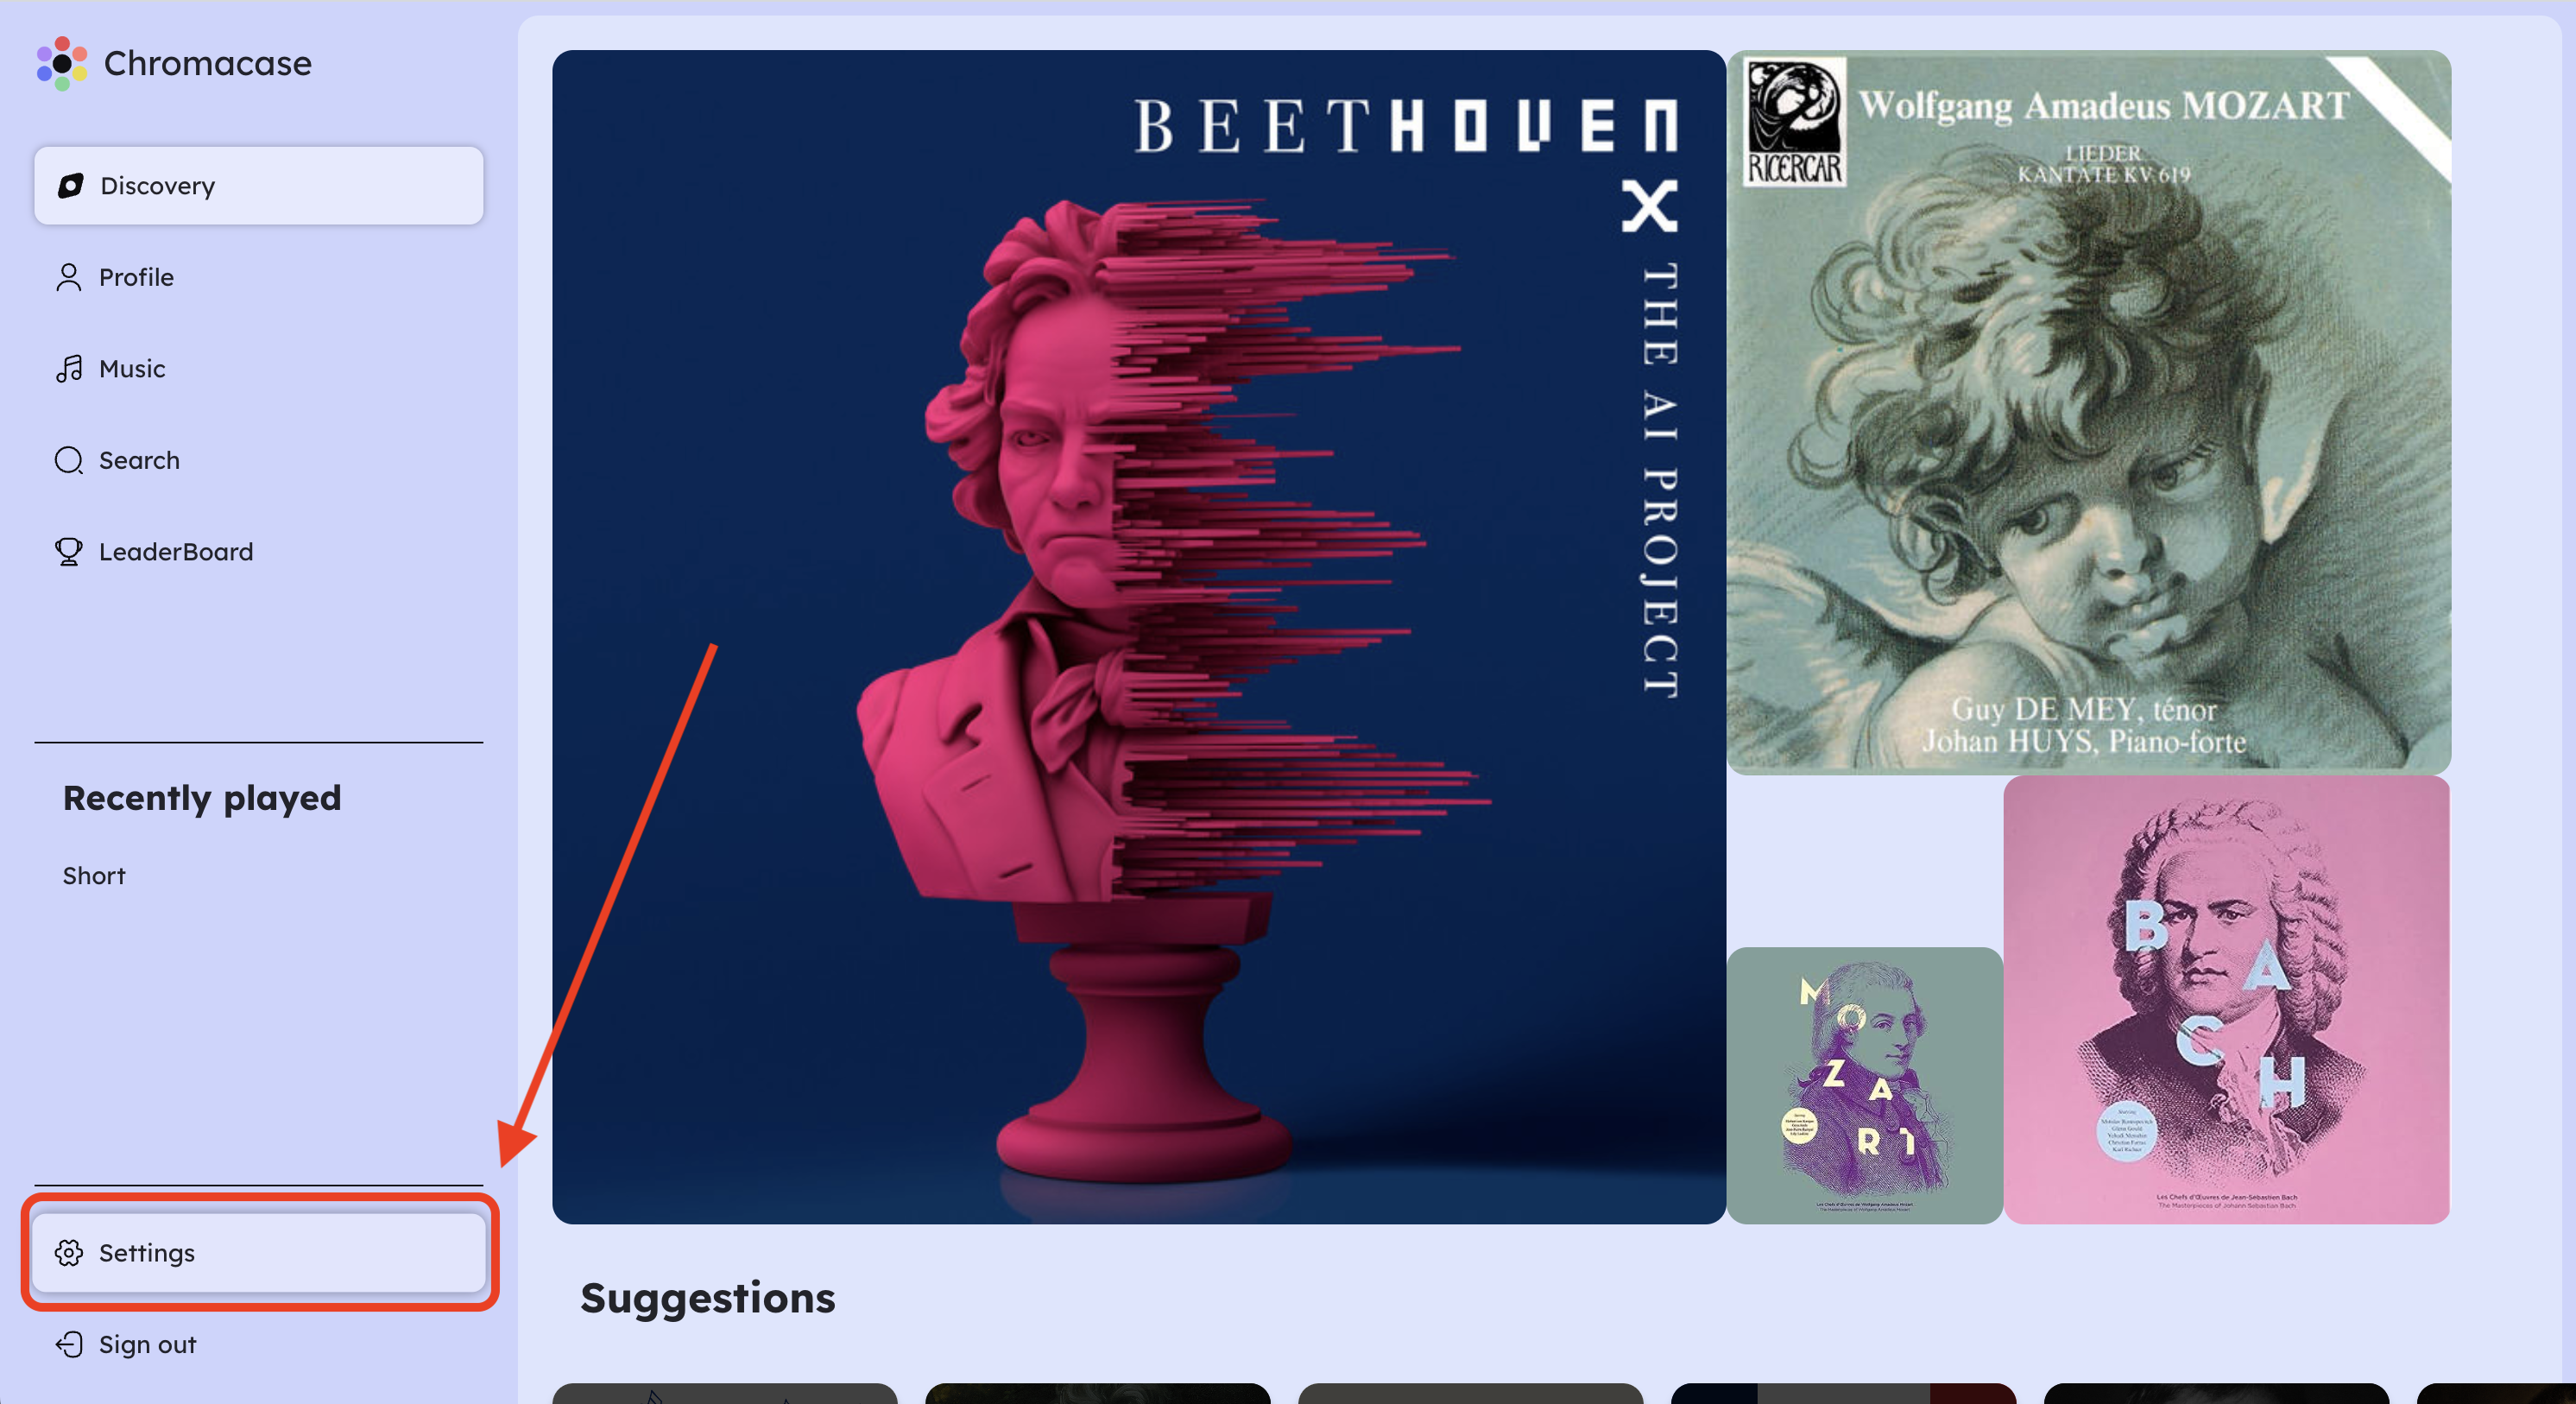
\includegraphics[width=\linewidth]{../\dir/guide/settings/access-settings.png}
		\caption{Version navigateur}
	\end{subfigure}
	\begin{subfigure}[b]{0.25\textwidth}
		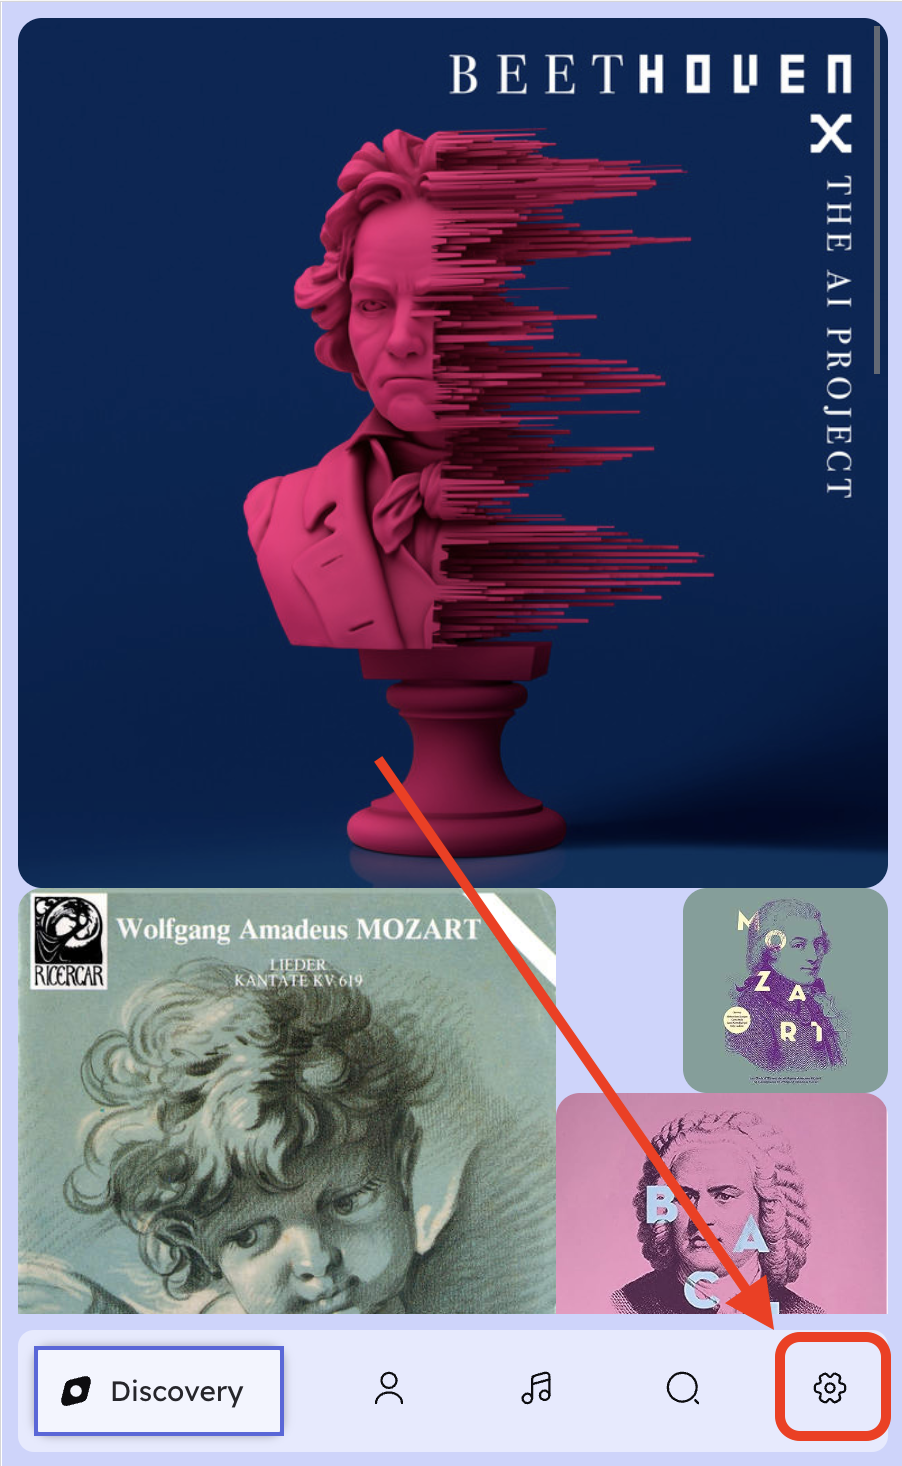
\includegraphics[width=\linewidth]{../\dir/guide/settings/access-settings-mobile.png}
		\caption{Version mobile}
	\end{subfigure}
	\caption{Acceder aux reglages}
	\label{fig:access-settings-lang}
\end{figure}

Sélectionnez l’onglet “Préférences”, et choisissez l’option de langue à utiliser (Voir Capture \ref{fig:change-language}).

\begin{figure}[H]
	\begin{subfigure}[b]{0.7\textwidth}
		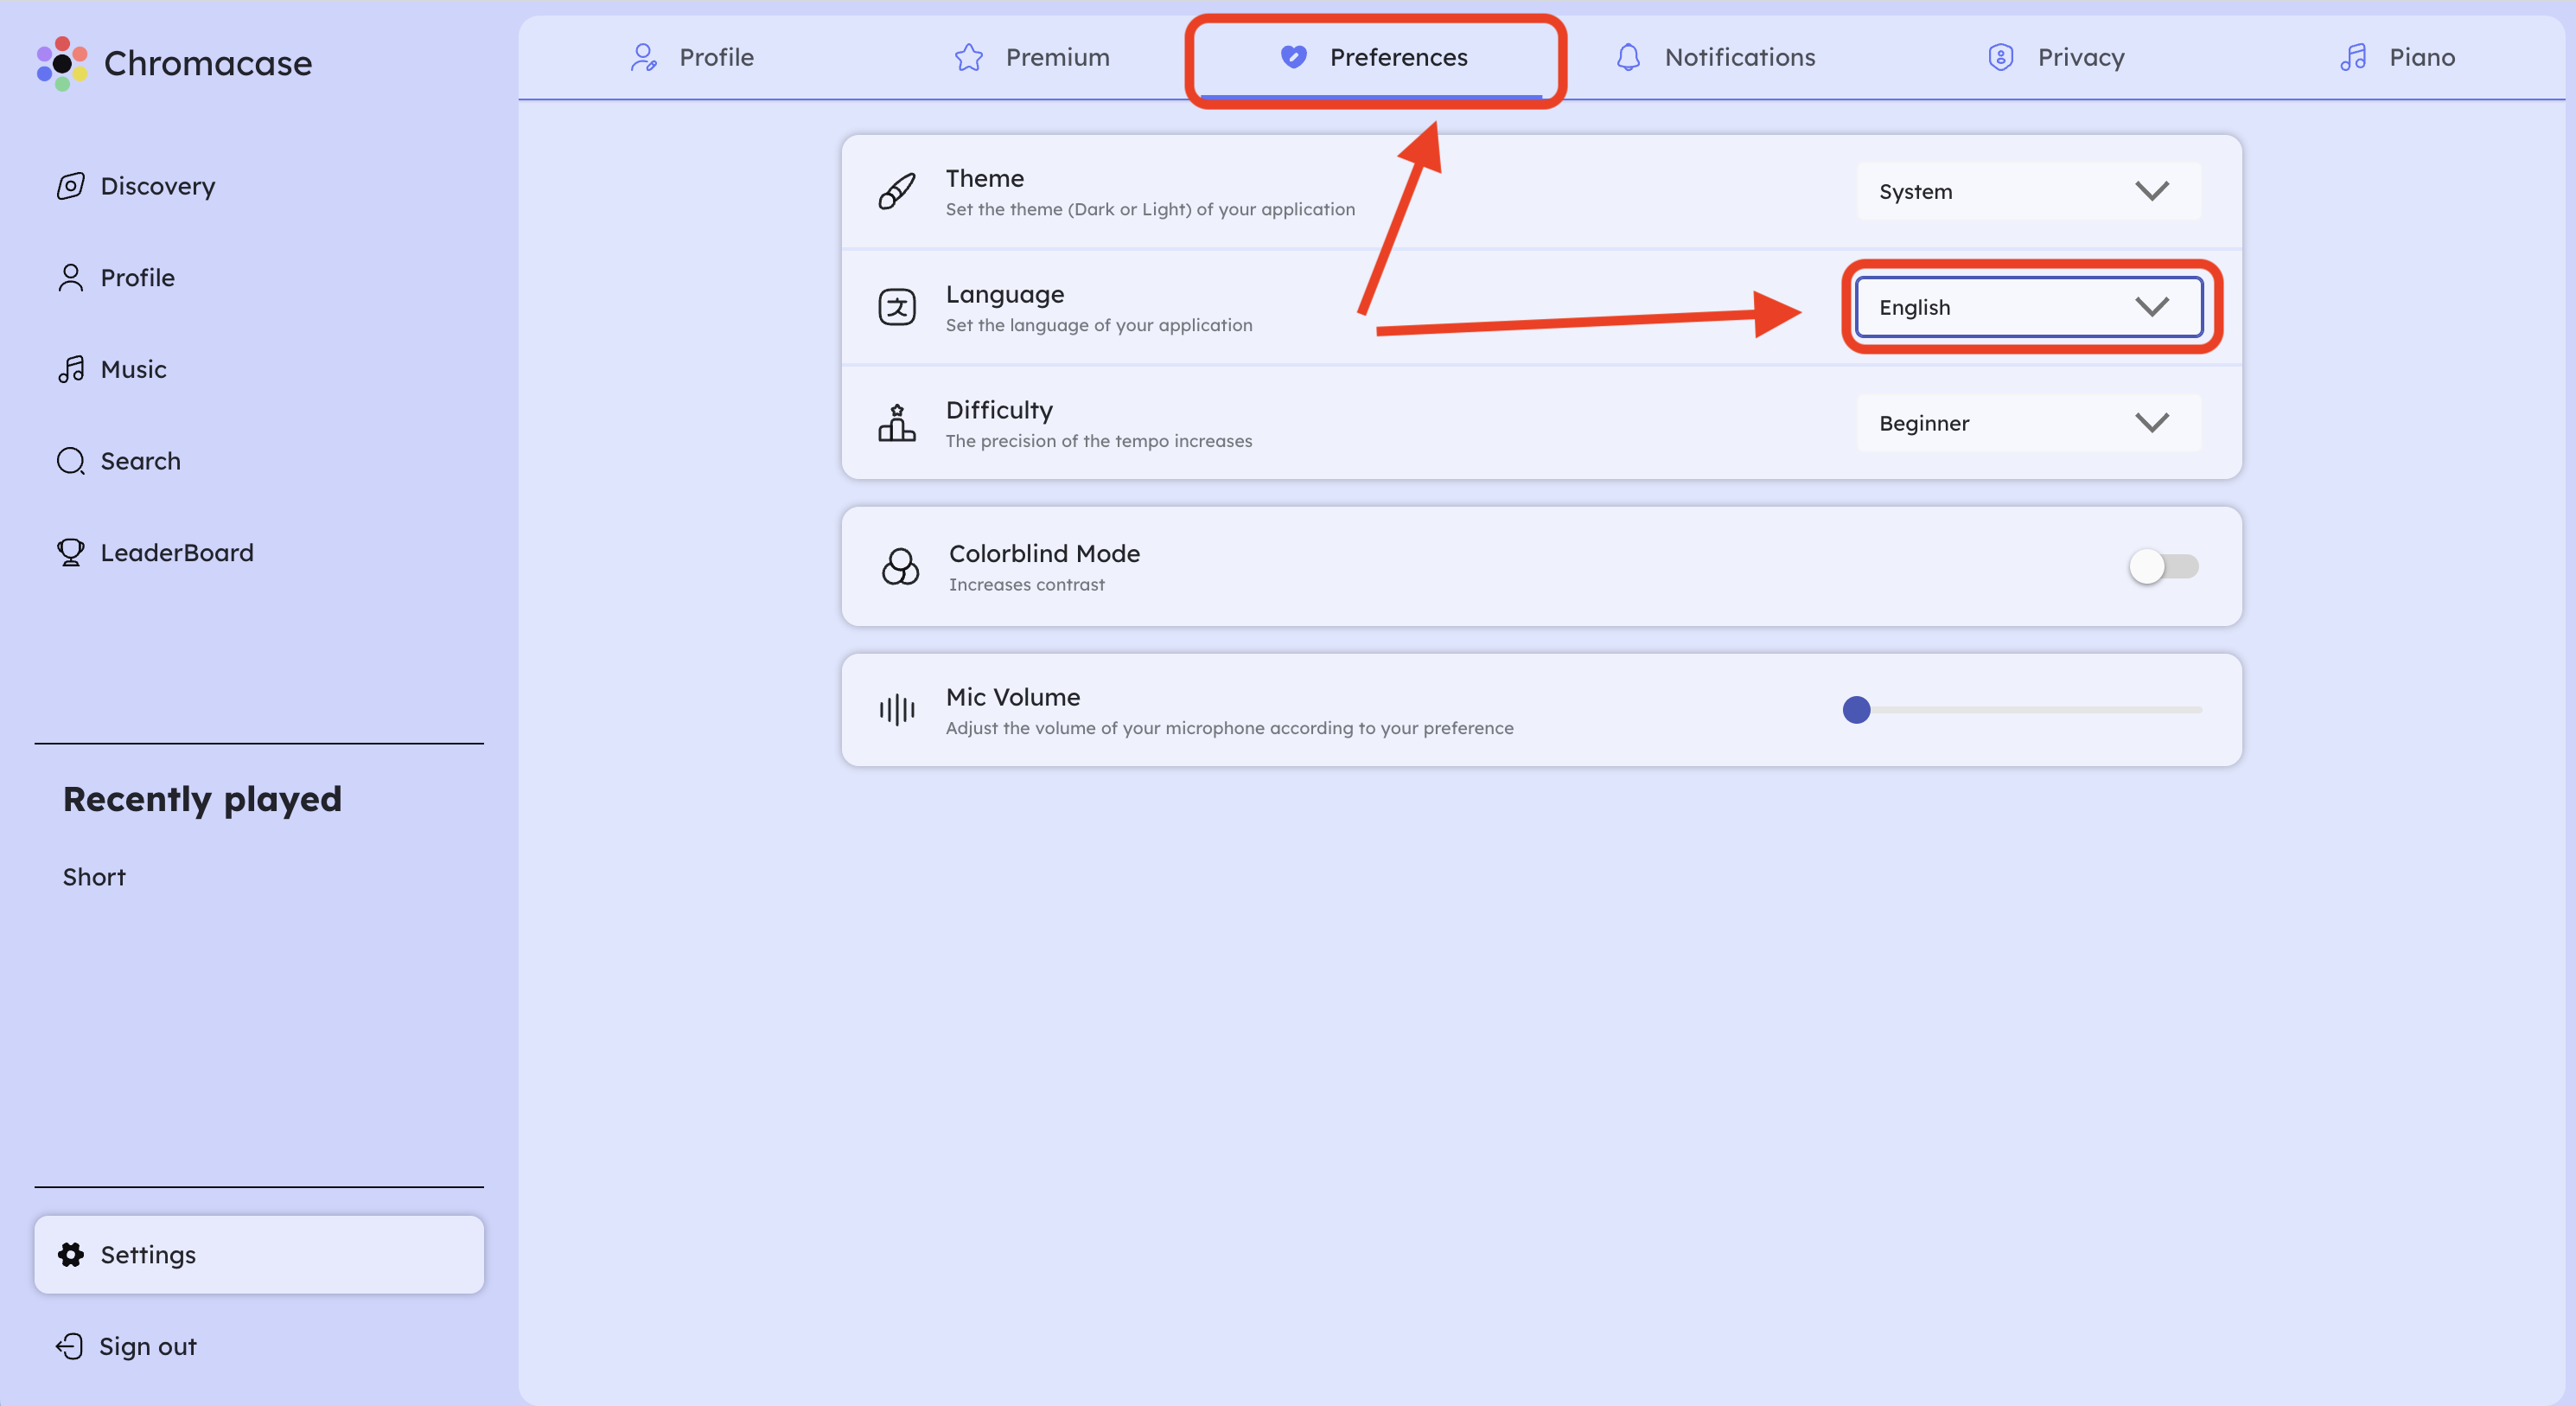
\includegraphics[width=\linewidth]{../\dir/guide/settings/change-language.png}
		\caption{Version navigateur}
	\end{subfigure}
	\begin{subfigure}[b]{0.25\textwidth}
		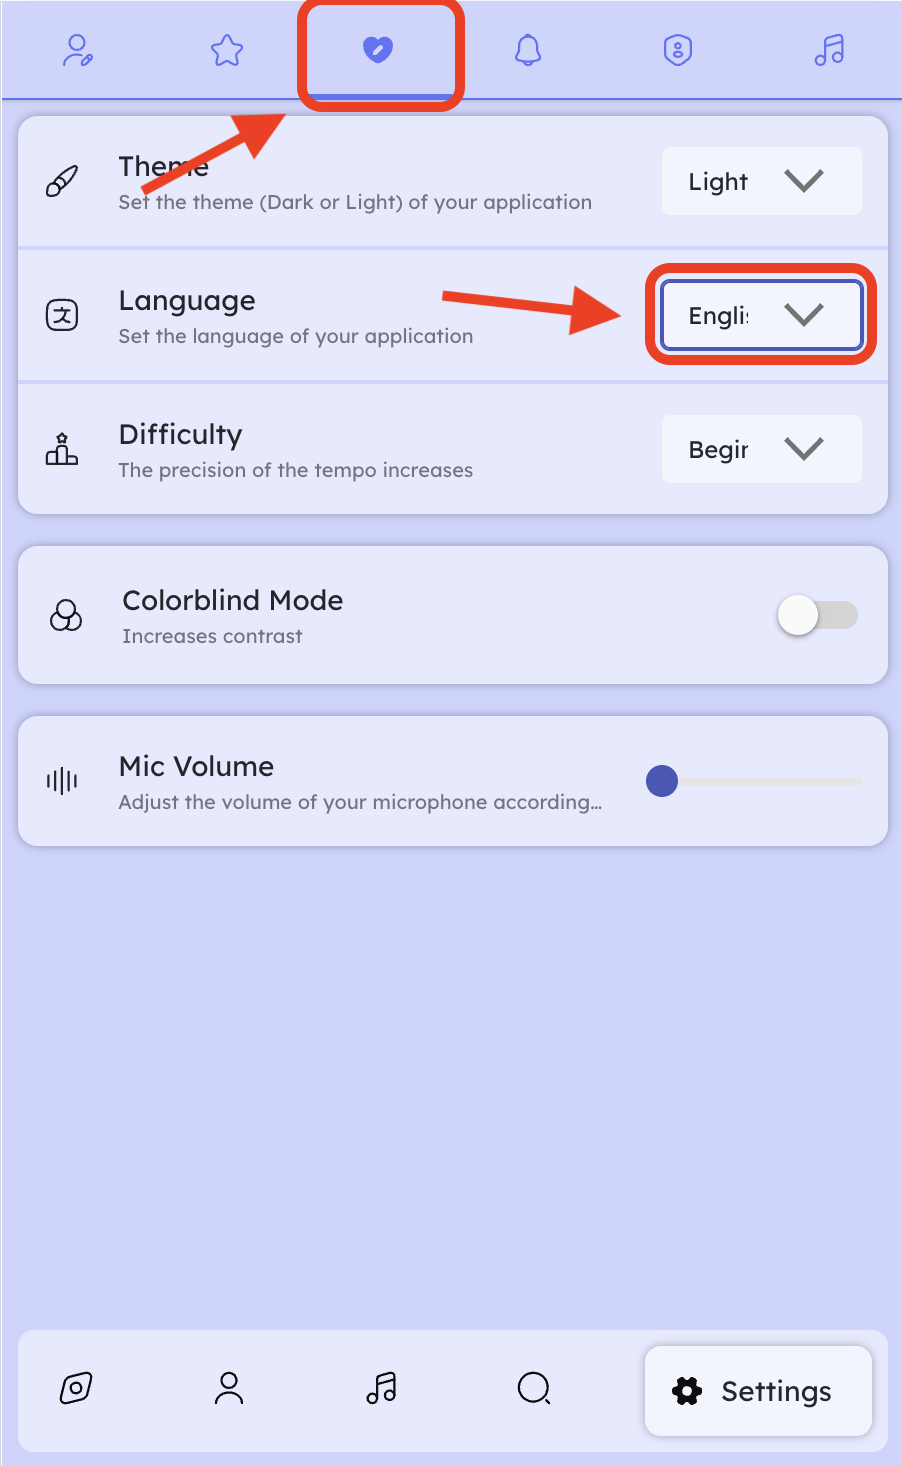
\includegraphics[width=\linewidth]{../\dir/guide/settings/change-language-mobile.png}
		\caption{Version mobile}
	\end{subfigure}
	\caption{Selectionner la langue}
	\label{fig:change-language}
\end{figure}
